% !TeX root = probability.tex

%%%%%%%%%%%%%%%%%%%%%%%%%%%%%%%%%%%%%%%%%%%%%%%%%%%%%%%%%%%%%%


\addcontentsline{toc}{section}{\large בחינות ופתרונות}

\section{קיץ תשפ"ב מועד ב}

\begin{center}
\selectlanguage{english}
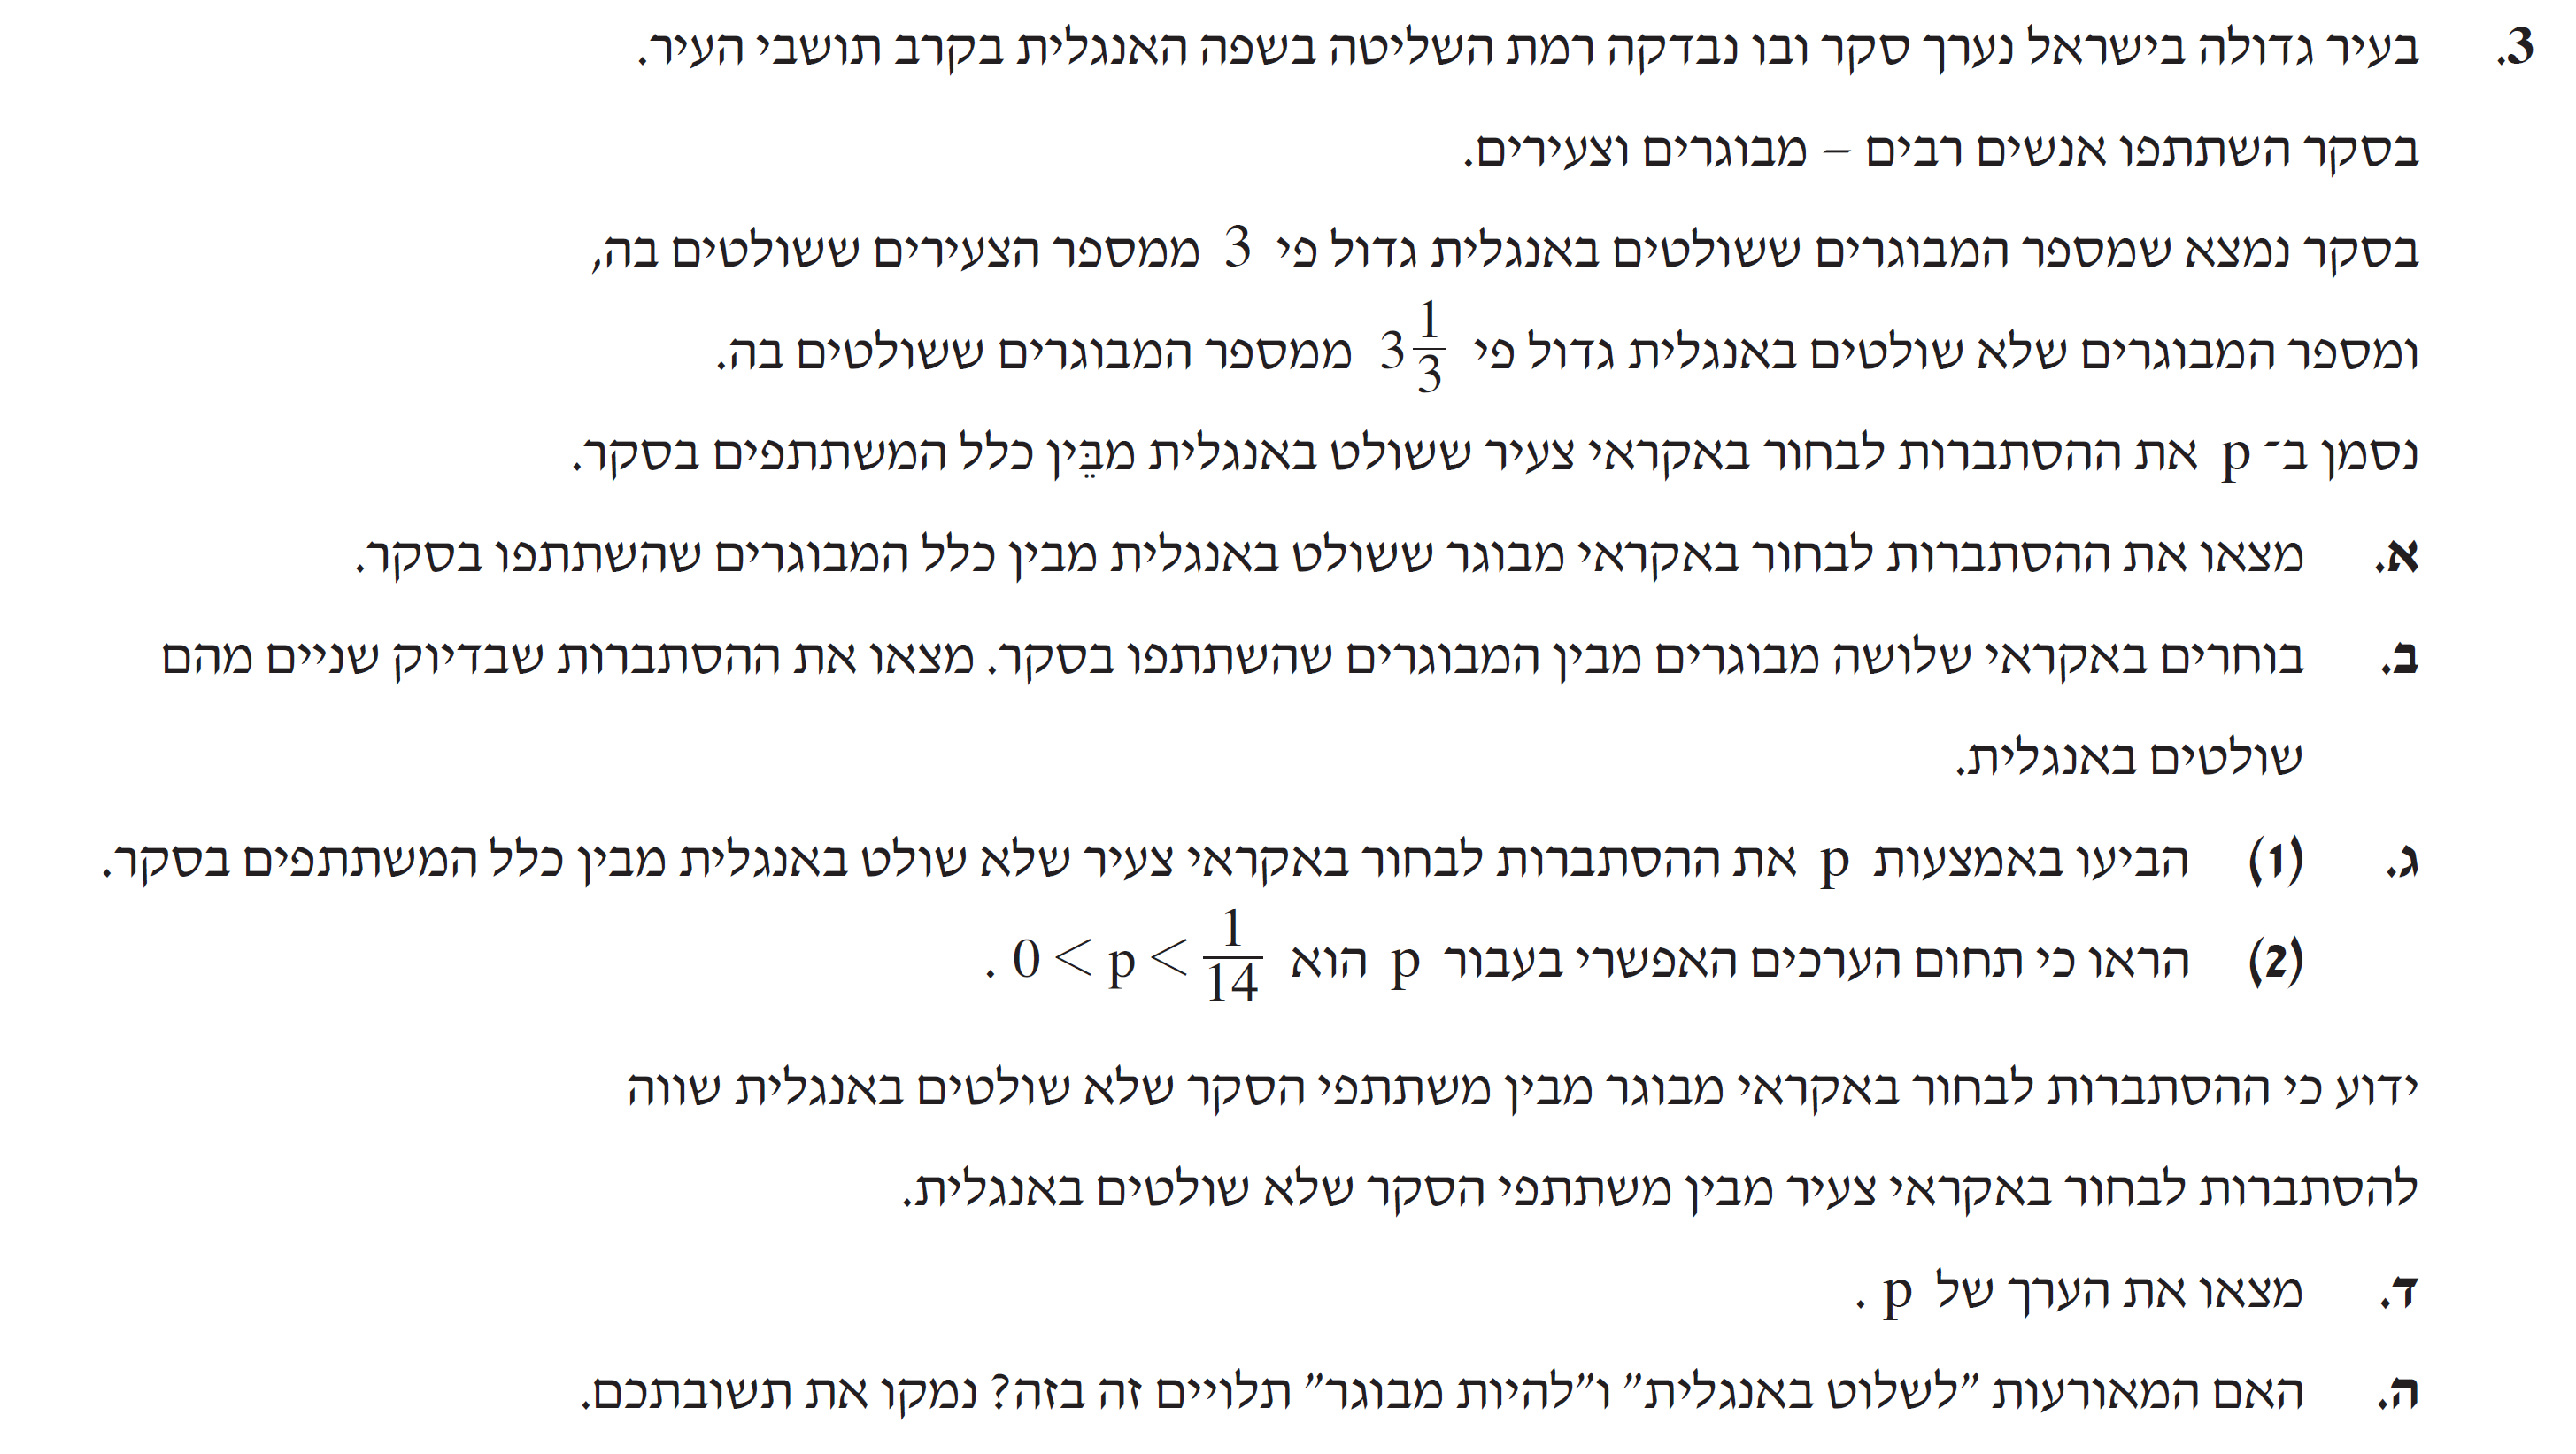
\includegraphics[width=\textwidth]{summer-2022b-3}
\end{center}

נסמן ב-%
$M$ \L{(mevugar)}
את המאורע של מבוגר ונסמן ב-%
$A$ \L{(anglit)}
את המאורע של שליטה באנגלית. השאלה שואלת על שני סוגים של מאורעות ולכן נארגן את המידע בטבלה. נתון הסימון
$p=P(\overline{M}\cap A)$.
\begin{quote}
אפשר לחשוב שניסוח "מבין" מכוון להסתברות מותנית, אבל בגלל שהניסוח "מבין כלל המשתתפים בסקר" מתייחס ל"כולם", אין אף משתתף שלא משתתף! אם רוצים אפשר לחשב הסתברות מותנית, כאשר נסמן את "כלל המשתתפים בסקר ב-%
$K$
ואז:
\begin{eqn}
P(K)&=&P(M\cup \overline{M})=P(A\cup \overline{A})=1\\
P((\overline{M}\cap A)/K)&=&
\frac{P((\overline{M}\cap A)\cap K)}{P(K)}=P(\overline{M}\cap A)\,.
\end{eqn}
\end{quote}

נתון גם ש-%
$P(M\cap A)=3P(\overline{M}\cap A)$
ולכן
$P(M\cap A)=p$,
ונתון ש-%
$P(M\cap \overline{A})=\frac{10}{9}P(M\cap A)$
ולכן
$P(M\cap \overline{A})=10p$.
ביחד עם ההסתברויות המשלימות נוכל למלא את כל התאים בטבלה.
\begin{center}
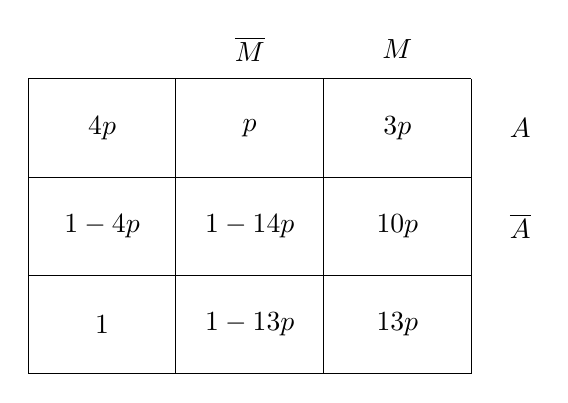
\begin{tikzpicture}[scale=1.25]
\draw (0,0) grid[xstep=1.5] (4.5,3);
\node at (3.75,3.3) {$M$};
\node at (2.25,3.3) {$\overline{M}$};
\node at (5,2.5) {$A$};
\node at (5,1.5) {$\overline{A}$};

\node at (3.75,2.5) {$3p$};
\node at (2.25,2.5) {$p$};
\node at (0.75,2.5) {$4p$};

\node at (3.75,1.5) {$10p$};
\node at (2.25,1.5) {$1-14p$};
\node at (0.75,1.5) {$1-4p$};

\node at (0.75,0.5) {$1$};
\node at (2.25,0.5) {$1-13p$};
\node at (3.75,0.5) {$13p$};
\end{tikzpicture}
\end{center}

\textbf{סעיף א}

\[
P(M\cap A/M)=\frac{P((M\cap A)\cap M)}{P(M)}=\frac{P(M\cap A)}{P(M)}=\frac{3p}{13p}=\frac{3}{13}\,,
\]
כי אם המשתתף נמצא ב-%
$M\cap A$
הוא כמובן נמצא גם ב-%
$M$.

\textbf{סעיף ב}

"מבין" מכוון להסתברות מותנית ו-"בדיוק" מכוון לנוסחת ברנולי. נשתשמש בתוצאה של הסעיף הקודם:
\[
P((M\cap A)=2/M=3)={3\choose 2}\left(\frac{3}{13}\right)^2
\left(\frac{10}{13}\right)^1=
\frac{270}{2197}=0.1229\,.
\]

\textbf{סעיף ג 1}

מהטבלה
$P(\overline{M}\cap A)=1-14p$.

\textbf{סעיף ג 2}

ההסתברות חייבת להיות בין אפס לאחד. מ-%
$0<1-14p$
מתקבל
$p<1/14$,
ומ-%
$1-14p<1$
מתקבל
$p>0/14=0$.

\textbf{סעיף ד}

כמו בדיון לעיל, "ידוע" לא מכוון להסתברות מותנית:
\begin{eqn}
P(M\cap \overline{A})&=&P(\overline{M}\cap \overline{A})\\
10p&=&1-14P\\
p&=&1/24\,.
\end{eqn}

\textbf{סעיף ה}

נבדוק אם
$P(M\cap A)=P(M)P(A)$:
\begin{eqn}
P(M\cap A)&=& 3p=3/24=1/8\\
P(M)P(A)&=&13p\cdot 4p=52/576=0.72/8\,.
\end{eqn}
הערכים שונים ולכן ההסתברויות תלויות זו בזו.

%%%%%%%%%%%%%%%%%%%%%%%%%%%%%%%%%%%%%%%%%%%%%%%%%%%%%%%%%%%%%

\newpage

\section{קיץ תשפ"ב מועד א}

\begin{center}
\selectlanguage{english}
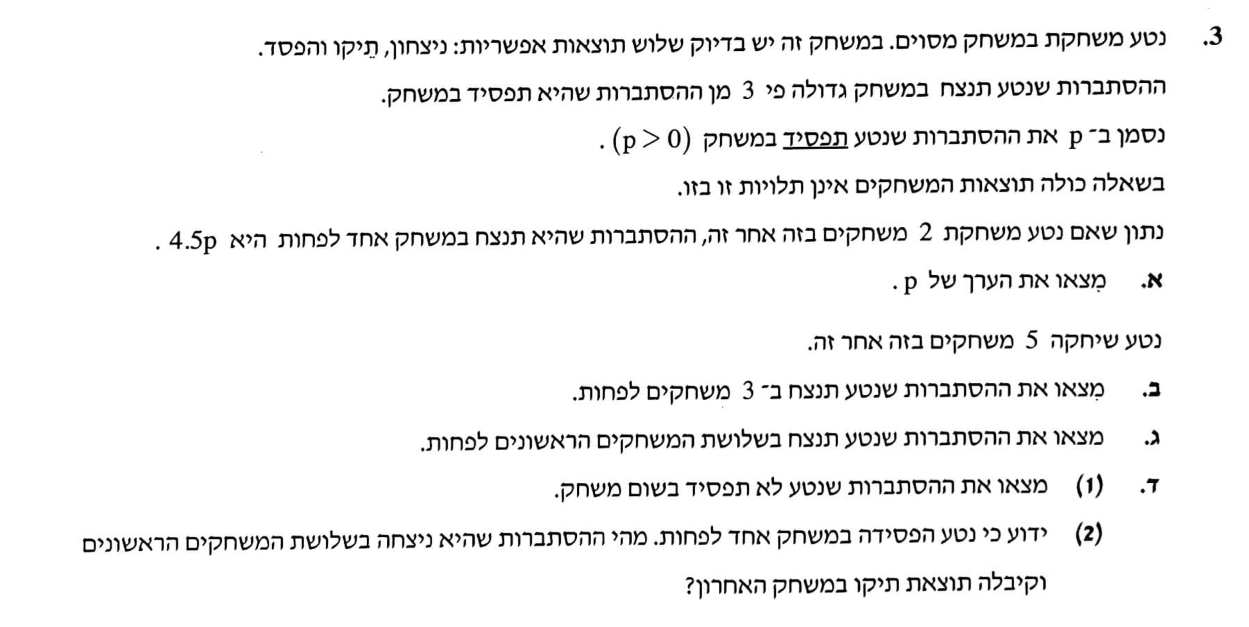
\includegraphics[width=\textwidth]{summer-2022a-3}
\end{center}

נסמן ב-%
$N$ \L{(nitzahon)},
$T$ \L{(teku)},
$H$ \L{(hefsade)}
את המאורעות של ניצחון, תיקו והפסד, בהתאמה. נתון ש-%
$P(H)=p$
ו-%
$P(N)=3p$.
לפי הסתברות משלימה
$P(T)=1-4p$.

\textbf{סעיף א}

ההסתברות לניצחון אחד לפחות היא המשלימה להסתברות לא לנצח פעמיים שהיא ההסתברות להפסד או תיקו פעמיים. לפי הנתון הסתברות זו היא
$4.5p$
ו-%
$p>0$:
\begin{eqn}
1-(p+(1-4p))^2&=&\tfrac{9}{2}p\\
1-(1-6p+9p^2)&=&\tfrac{9}{2}p\\
9p^2&=&\tfrac{3}{2}p\\
p&=&\tfrac{1}{6}\,.
\end{eqn}
מכאן ש-%
$P(N)=\frac{1}{2}, P(T)=\frac{1}{3}$.

\textbf{סעיף ב}

"לפחות" מכוון לנוסחת ברנולי. שימו לב שכאשר ההסתברות היא 
$\frac{1}{2}$:
\[
\left(\frac{1}{2}^k\right)\left(1-\frac{1}{2}\right)^{n-k}=\left(\frac{1}{2}\right)^n\,,
\]
ולכן ההסתברות היא סכום המקדמים הבינומיים כפול 
$\left(\frac{1}{2}\right)^5$:
\[
P(N=3)=\frac{1}{32}\left({5\choose 3}+{5\choose 4}+{5\choose 5}\right)=\frac{16}{32}=\frac{1}{2}\,.
\]

\textbf{סעיף ג}

ההסתברות המבוקשת היא ההסתברות לנצח בשלושה משחקים ברציפות שהיא
$\left(\frac{1}{2}\right)^2=\frac{1}{8}$
כפול ההסתברות לניצחון או תיקו או הפסד בשני משחקים ברציפות שהיא
$1\cdot 1$,
כי שלושת התוצאות הללו מכסות את כל האפשריות. לכן התשובה היא
$\frac{1}{8}$.

\textbf{סעיף ד 1}

ההסתברות שנטע לא תפסיד היא
$1-\frac{1}{6}=\frac{5}{6}$,
ההסתברות המשלימה להסתברות שהיא תפסיד. ההסתברות המבוקשת היא:
\[
P(\overline{H}=5)=\left(\frac{5}{6}\right)^5=\frac{3125}{7776}=0.4019.
\]

\textbf{סעיף ד 2}

מאוד מפתה להבין את השאלה בצורה מוטעית: אם נטע מנצחת בשלושת המשחקים הראשונים ומשיגה תיקו בחמישי, אין ברירה אלא שהיא תפסיד את הרביעי וההסתברות היא:
\[
\left(\frac{1}{2}\right)^3\cdot \frac{1}{6}\cdot \frac{1}{3}=\frac{1}{144}\,.
\]
אבל "ידוע" מכוון להסתברות מותנית וההסתברות שחישבנו מתייחס לחלק מכל התוצאות האפשריות ולא רק מאלו שנטע הפסידה משחק אחד לפחות. ההסתברות המבוקשת היא:
\[
P(N=1,N=2,N=3,T=5/H\geq 1)=\frac{P(N=1,N=2,N=3,T=5\cap H\geq 1)}{P(H\geq 1)}\,.
\]
המונה היא ההסתברות
$\frac{1}{144}$
שבדיוק חישבנו והמכנה הוא ההסתברות
$\frac{3125}{7776}$
שחישבנו בסעיף ד 1. ההסתברות המבוקשת היא:
\[
P(N=1,N=2,N=3,T=5/H\geq 1)=\frac{1/144}{3125/7776}=
\frac{7776}{144\cdot 4651}=\frac{54}{4651}=0.0116\,.
\]

%%%%%%%%%%%%%%%%%%%%%%%%%%%%%%%%%%%%%%%%%%%%%%%%%%%%%%%%%

\newpage

\section{חורף תשפ"ב}

\begin{center}
\selectlanguage{english}
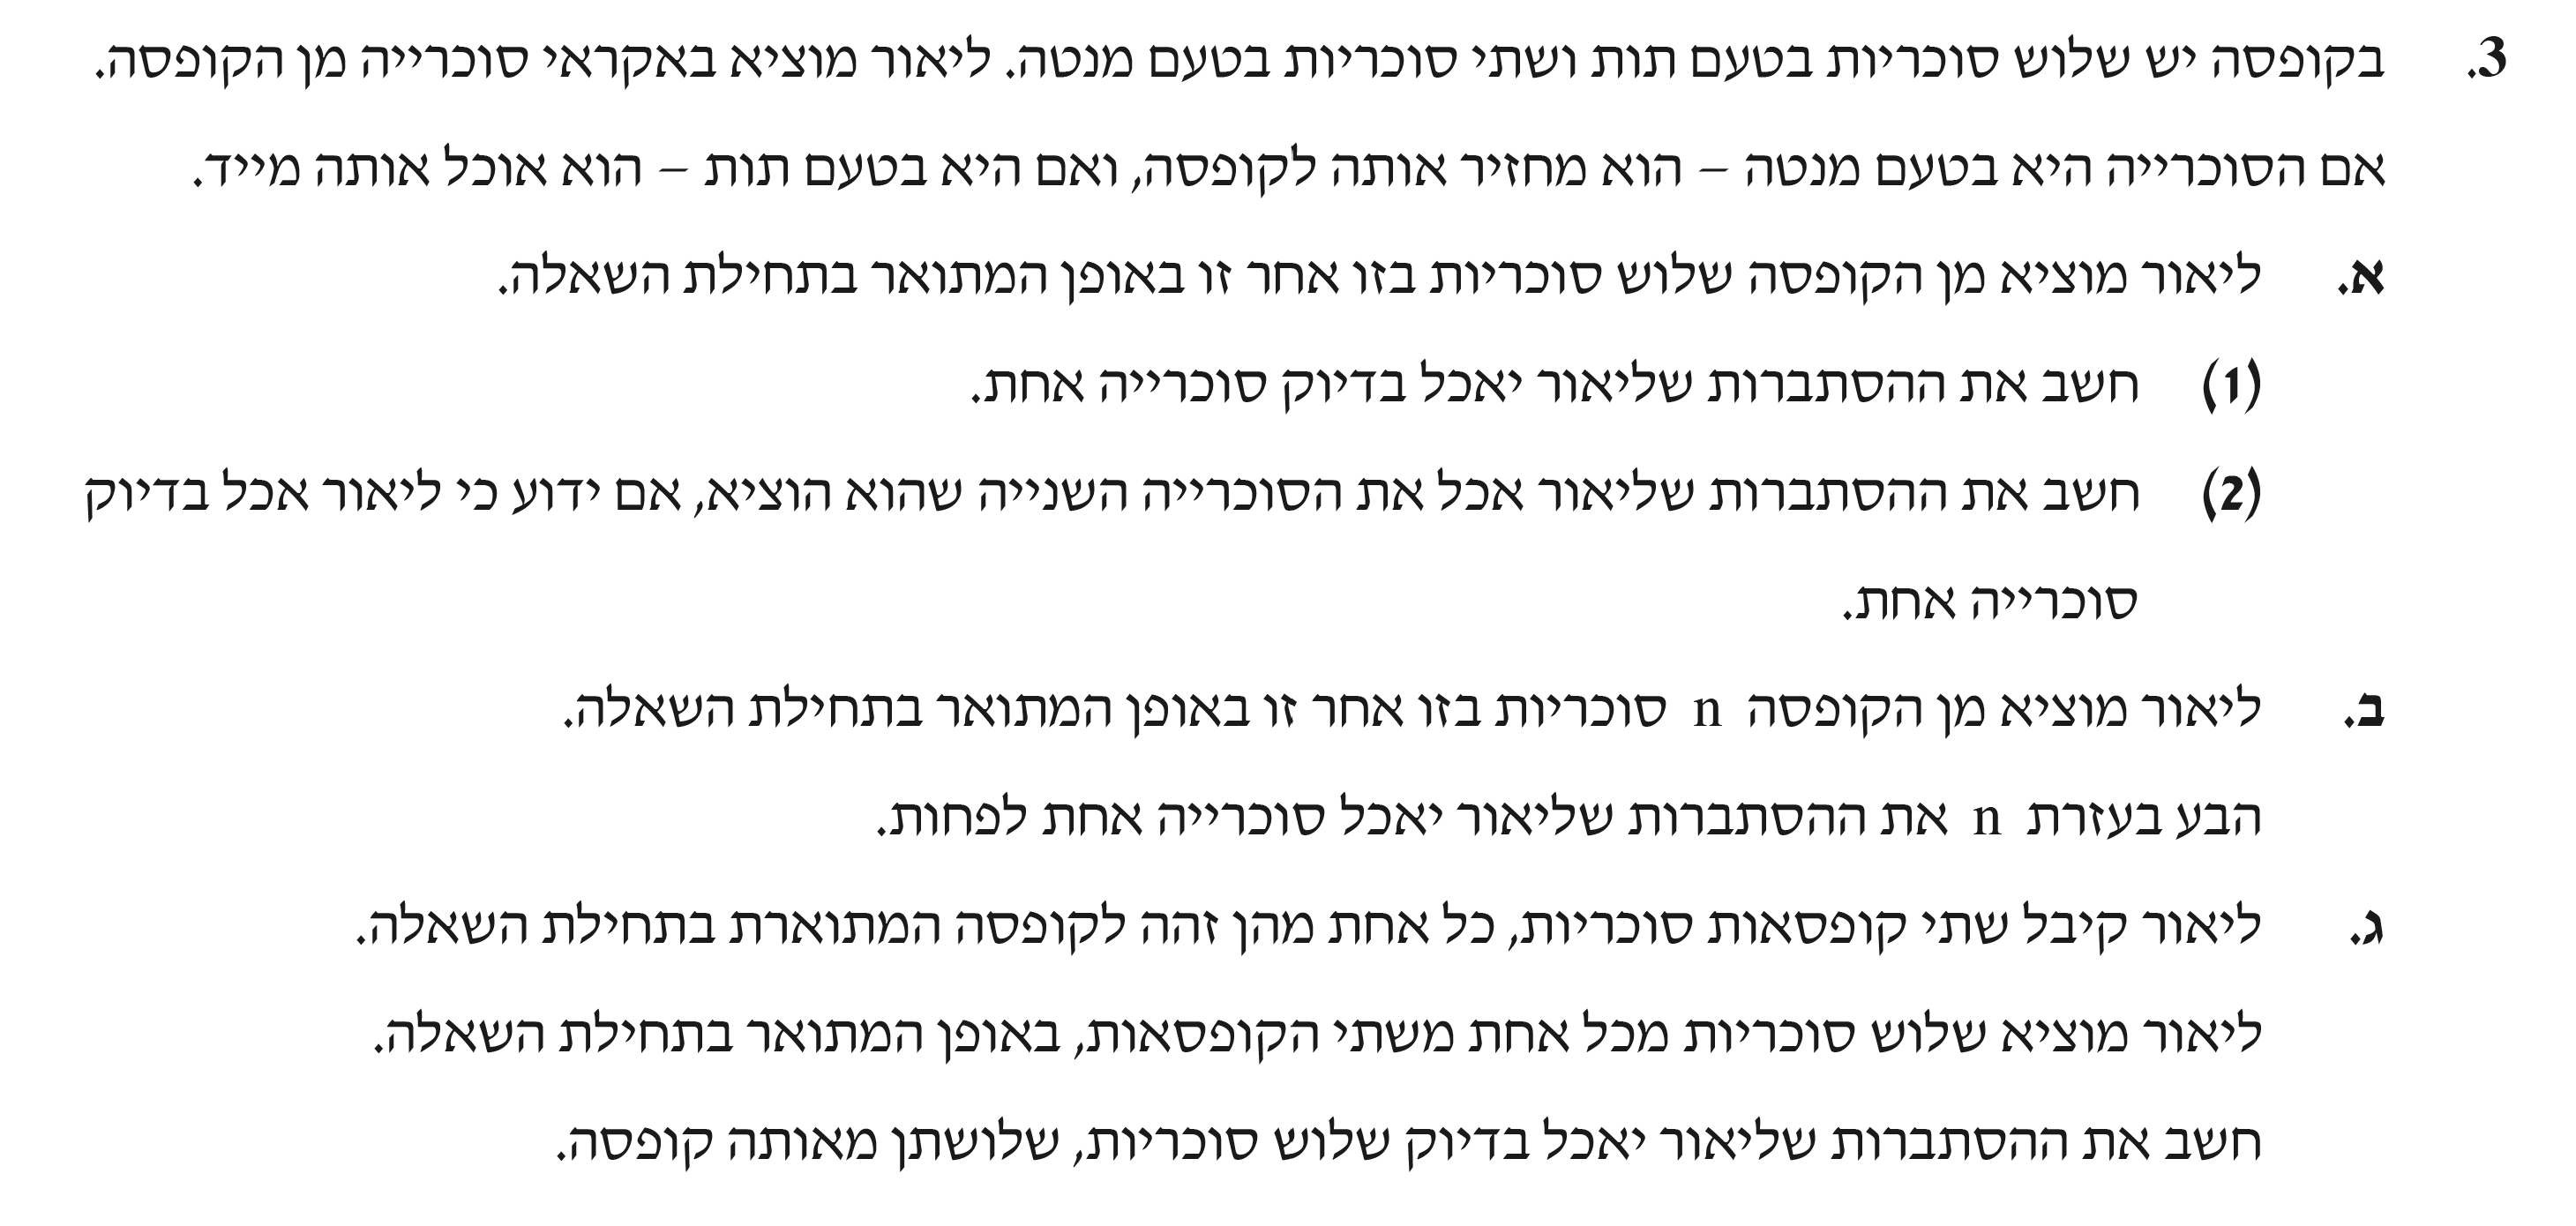
\includegraphics[width=\textwidth]{winter-2022-3}
\end{center}

השאלה שואלת על סדרה של מאורעות ולכן נארגן את המידע בעץ. בצמתים מוסמנים במספר הסוכריות באותו מצב
$(T, M)$,
והקשתות מסומנות בסוג הסוכריה שנשלף וההסתברותה.

\begin{center}
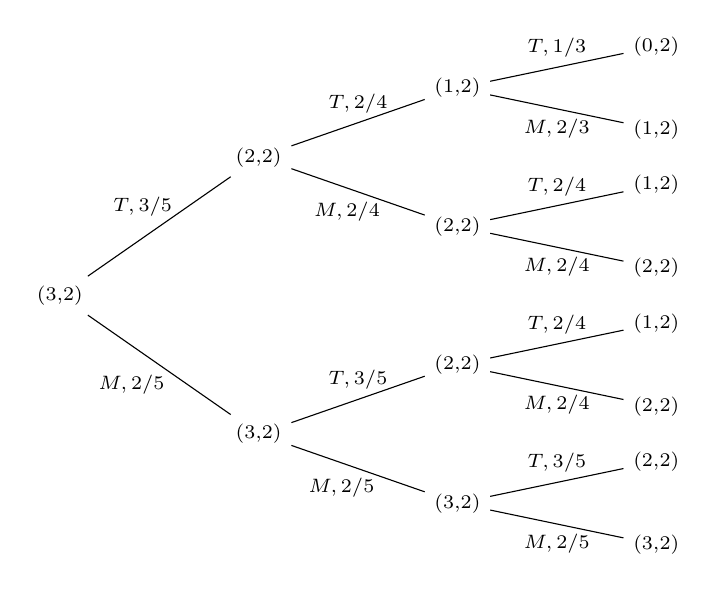
\begin{tikzpicture}
  [grow=right,
   level 1/.append style=
     {level distance=6em,sibling distance=10em},
   level 2/.append style=
     {level distance=6em,sibling distance=5em},
   level 3/.append style=
     {level distance=6em,sibling distance=3em}
  ]
  \node[left] {$\scriptstyle (3,2)$}
    child {node [right] {$\scriptstyle (3,2)$}
      child {node[right]  {$\scriptstyle (3,2)$}
        child {node[right]  {$\scriptstyle (3,2)$}
            edge from parent
            node [below] {$\scriptstyle M,\,2/5$}
        }
        child {node[right] {$\scriptstyle (2,2)$}
            edge from parent 
            node [above] {$\scriptstyle T,\,3/5$}
        }
        edge from parent
        node [below,xshift=-6pt] {$\scriptstyle M,\,2/5$}
      }
      child {node[right]  {$\scriptstyle (2,2)$}
        child {node[right]  {$\scriptstyle (2,2)$}
            edge from parent 
            node [below] {$\scriptstyle M,\,2/4$}
        }
        child {node[right] {$\scriptstyle (1,2)$}
            edge from parent
            node [above] {$\scriptstyle T,\,2/4$}
        }
        edge from parent
        node [above] {$\scriptstyle T,\,3/5$}
      }
      edge from parent
      node [below,,xshift=-10pt] {$\scriptstyle M,\, 2/5$}
    }
    child {node [right] {$\scriptstyle (2,2)$}
      child {node[right]  {$\scriptstyle (2,2)$}
        child {node[right]  {$\scriptstyle (2,2)$}
            edge from parent 
            node [below] {$\scriptstyle M,\,2/4$}
        }
        child {node[right] {$\scriptstyle (1,2)$}
            edge from parent 
            node [above] {$\scriptstyle T, \,2/4$}
        }
        edge from parent
        node [below,xshift=-4pt] {$\scriptstyle M,\, 2/4$}
      }
      child {node[right]  {$\scriptstyle (1,2)$}
        child {node[right]  {$\scriptstyle (1,2)$}
            edge from parent 
            node [below] {$\scriptstyle M, \,2/3$}
        }
        child {node[right] {$\scriptstyle (0,2)$}
            edge from parent 
            node [above] {$\scriptstyle T,\, 1/3$}
        }
        edge from parent node [above] {$\scriptstyle T,\, 2/4$}
      }
      edge from parent
      node [above,xshift=-6pt] {$\scriptstyle T, \,3/5$}
    };
\end{tikzpicture}
\end{center}

\textbf{סעיף א 1}

הניסוי מתחיל עם שלוש סוכריות. ליאור אוכל רק סוכריות תות ולכן ההסתברות שהוא יאכל רק אחת היא סכום ההסתברויות לאורך המסלולים המובילים למצבים המסומנים
$(2,k)$.

אם הוא שוךף סוכריית מנטה הוא לא יאכל אותה ולכן חייב להיות
$k=2$.
יש שלושה מסלולים, הרביעית, ששית ושביעית (מלמעלה):
\begin{eqn}
P((2,2))&=&
\frac{3}{5}\cdot\frac{2}{4}\cdot\frac{2}{4}+
\frac{2}{5}\cdot\frac{3}{5}\cdot\frac{2}{4}+
\frac{2}{5}\cdot\frac{2}{5}\cdot\frac{3}{5}=\frac{183}{500}=0.366\,.
\end{eqn}

\textbf{סעיף א 2}

נסמן ב-%
$A$ \L{(akhal)}
את המאורע של אכילת סוכרייה. "ידוע" מכוון להסתברות מותנית. אנחנו עדיין במצב של שליפת שלוש סוכריות ולכן אכילת הסוכרייה השנייה אפשרית רק לאורך המסלול 
$MTM$.
אם ליאור שלף הסוכריית תות בשליפה השנייה, קל וחומר שהוא אכל סוכרייה כלשהי, ולכן
$A=1\subseteq MTM$.
מהתוצאה של הסעיף הקודם ונקבל:
\[
P(MTM/A=1)=\frac{P(MTM\cap (A=1))}{P(A=1)}=\frac{P(MTM)}{P(A=1)}=
\frac{3/25}{183/500}=\frac{20}{61}=0.3279\,.
\]

\textbf{סעיף ב}

"בזו אחר זו" מכוון להתפלגות בינומית. הנוסחה מסובכת אלא אם נחשב את ההסתברות המשלימה:
\[
P(A\geq 1)=1-P(A=0)=1-\left(\frac{2}{5}\right)^n\,.
\]

\textbf{סעיף ג}

ההסתברות היא הסתברות לשלוף שלוש סוכריות תות מהקופסה אחת ושלוש סוכריות מנטה מהקופסה השנייה. נפלתי בפח כאן: איך אני יכול לשלוף שלוש סוכריות מנטה מקופסה שיש לה שתי סוכריות מנטה? צריך כמובן לזכור שהשליפה של סוכריות מנטה היא עם החזרה. ההסתברות המבוקשת מתקבלת מהמסלול העליון בעץ כפול התחתון בעץ כפול שניים כי אפשר לבחור את הקופסאות בשתי דרכים:
\[
P(T=3,M=3)=2\left(\frac{3}{5}\cdot\frac{2}{4}\cdot\frac{1}{3}\right)
\left(\frac{2}{5}\right)^3=2\cdot\frac{3}{30}\cdot\frac{8}{125}=
\frac{8}{625}=0.0128\,.
\]

%%%%%%%%%%%%%%%%%%%%%%%%%%%%%%%%%%%%%%%%%%%%%%%%%%%%%%%%%

\newpage

\section{חורף תשפ"ב מועד נבצרים}

\begin{center}
\selectlanguage{english}
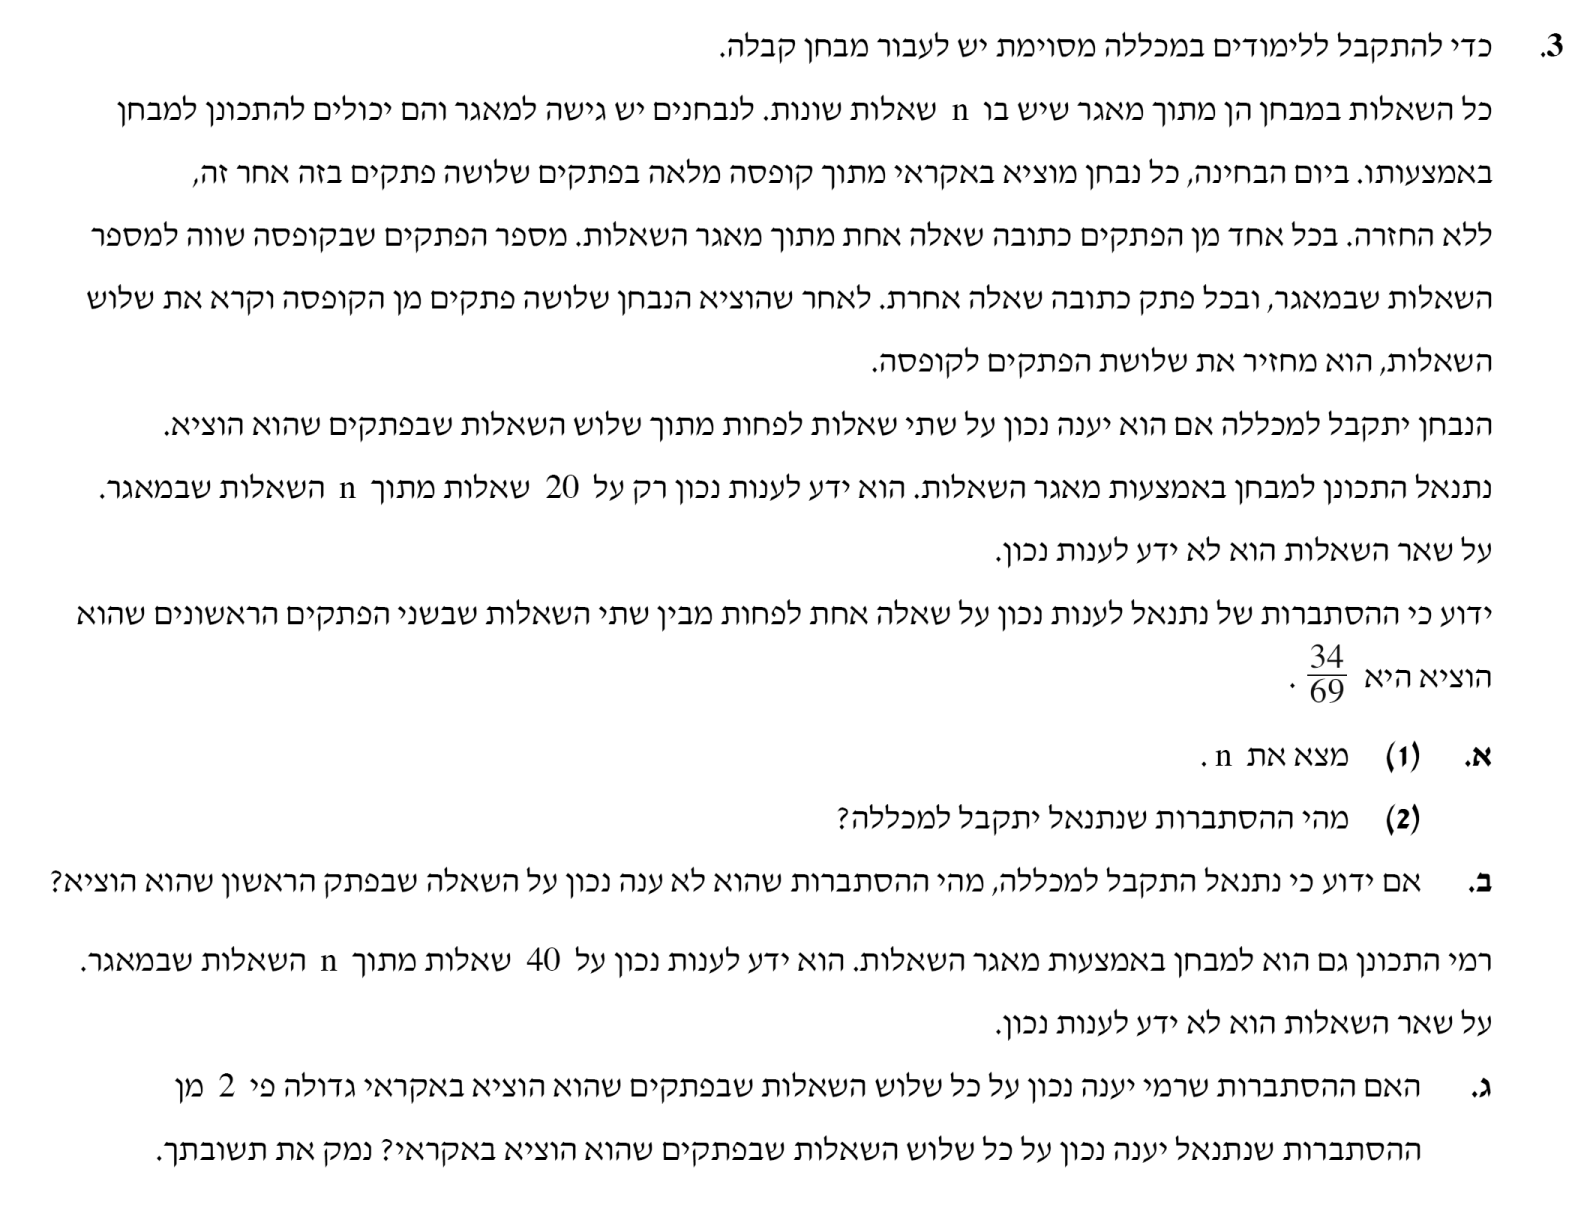
\includegraphics[width=\textwidth]{winter-2022nv-3}
\end{center}

לדעתי ניסוח השאלה ארוכה מדי!

"ידוע כי ההסתברות" לא מכוון להסתברות מותנית. בסעיף א 1 שום מאורע לא תלוי במאורע שנתנאל "ענה נכון
$\ldots$",
אלא פשוט נתונה ההסתברות של המאורע. לדעתי ניתן לפרש את סעיף א 2 כמבקשת את ההסתברות נתנאל יתקבל למכללה "אם ידוע כי 
$\ldots$".
בבדיקת פתרונות באינטרנט לא מצאתי אף אחד שחשב כמוני.

\textbf{סעיף א 1}

התשובה יחסית פשוטה למצוא אבל החישובים מסובכים ולא האמנתי שייצא מהם משהו. נסמן ב-%
$N$ \L{(nachon)}
את המאורע שנתנאל ענה נכון. "לפחות" מכוון להתפלגות בינומית. נחשב את ההסתברות המשלימה כאשר יש להקפיד שהשליפות הן ללא החזרה:
\begin{eqn}
P(N\geq 1)&=&1-\frac{n-20}{n}\cdot\frac{n-20}{n-1}=
\frac{34}{69}\\
\frac{40n-420}{n^2-n}&=&\frac{34}{69}\\
17n^2-1397n+14490&=&0\\
n&=&\frac{1397\pm 983}{34}=70,\, 20.3\,.
\end{eqn}
מספר השאלות הוא מספר שלם ולכן התשובה היא
$70$.

\textbf{סעיף א 2}

כדי להתקבל למכללה נתנאל חייב לענות נכון על שאלות: (א) 
$1,2,3$
או (ב)
$1,2$
או (ג)
$1,3$
או (ד)
$2,3$.

נסמן ב-%
$Y$ \L{(yitkabel)}
את המאורע שהוא יתקבל למכללה. ההסתברות המבוקשת היא:
\begin{eqn}
P(Y)&=&
\frac{20}{70}\cdot\frac{19}{69}+
\frac{20}{70}\cdot\frac{50}{69}\cdot\frac{19}{68}+
\frac{50}{70}\cdot\frac{20}{69}\cdot\frac{19}{68}\\[8pt]
&=&\frac{20\cdot 19\cdot (68+50+50)}{70\cdot 69\cdot 68}=
\frac{76}{391}=0.1944\,.
\end{eqn}
ויתרתי על החישוב של ההסתברות של מאורע (א) כי הוא כלול במאורע (ב). אם מתעקשים אפשר לחשב:
\[
\frac{20}{70}\cdot\frac{19}{69}\cdot\frac{18}{68} + \frac{20}{70}\cdot\frac{19}{69}\cdot \frac{50}{68}=\frac{20}{70}\cdot\frac{19}{69}=\frac{20}{70}\cdot\frac{19}{69}\left(\frac{18}{68}+\frac{50}{68}\right)=\frac{20}{70}\cdot\frac{19}{69}\,.
\]

\textbf{סעיף ב}

ההסתברות המבוקשת היא:
\[
P(\overline{N}/Y)=\frac{P(\overline{N}\cap Y)}{P(Y)}\,.
\]
$P(\overline{N}\cap Y)$
היא הגורם השלישי בחישוב של 
$P(Y)$
בסעיף הקודם ו-%
$P(Y)$
היא התשובה מהסעיף הקודם, לכן:
\begin{eqn}
P(\overline{N}\cap Y)&=&
\frac{\disfrac{50}{70}\cdot\disfrac{20}{69}\cdot\disfrac{19}{68}}
{\disfrac{76}{391}}=\frac{50\cdot 20\cdot 19\cdot 191}{76\cdot 70\cdot 69\cdot 68}=\frac{25}{84}=0.2976\,.
\end{eqn}
בצימצום השבר אפשר להשתמש בפירוקים
$76=4\cdot 19$
ו-%
$391=17\cdot 23$.

\textbf{סעיף ג}

נסמן ב-%
$T=3$ \L{(neTanel)}
את המאורע שנתנאל ענה נכון על שלושת השאלות ונסמן ב-%
$R=3$ \L{(Rami)}
את המאורע שרמי ענה נכון על שלושת השאלות. נשווה את ההסתברויות:
\begin{eqn}
P(R=3)&\stackrel{?}{=}&2P(T=3)\\[8pt]
\frac{40}{70}\cdot\frac{39}{69}\cdot\frac{38}{68}
&\stackrel{?}{=}&
2\cdot\frac{20}{70}\cdot\frac{19}{69}\cdot\frac{18}{68}\\[8pt]
39 &\neq& 9\,,
\end{eqn}
והתשובה היא לא.
